% 第9章第4节：泛函极小值的存在（最小化序列、直接法、闭凸集投影）。

\section{泛函极小值的存在}
\label{sec:opt-fn-existence}

前两节的条件都以“最小点已经存在”为前提。有限维中，连续目标在非空紧集上必有最小点，第~\ref{chap:optimization}章用这一点处理了许多问题；无限维中闭有界集一般不紧，这条路走不通。本节从目标值越来越低的函数列出发，研究能否取到一个仍然可行、目标值不高于下确界的极限，并用闭凸集上的投影给出一个完整的例子。

\subsection{最小化序列}
\label{sec:opt-fn-minimizing-sequence}

设$C$非空，$m=\inf_{u\in C}J(u)$。由下确界的定义，总能选出$u_n\in C$使$J(u_n)\to m$，称$(u_n)$为\term{最小化序列}（minimizing sequence）。最小值是否达到，归结为能否从这样的序列中取出某种极限，并让极限保住两件事：仍在$C$中，目标值不超过$m$。

\paragraph{有界、连续，仍取不到下确界}
在$\ell^2$上取
\[
 J(\bm x)=\bigl(\|\bm x\|_2^2-1\bigr)^2+\sum_{k=1}^\infty\frac{x_k^2}k .
\]
$J$连续，$J\ge0$，并且$J(\bm x)\le c$推出$\|\bm x\|_2^2\le1+\sqrt c$，下水平集有界。沿标准单位向量，$J(\bm e_k)=1/k\to0$，所以$m=0$。可是$J(\bm x)=0$要求第二项为零即$\bm x=0$，此时第一项为$1$，下确界取不到。最小化序列$\bm e_k$两两相距$\sqrt2$，没有任何范数收敛的子列；在有限维中，闭有界集里的序列总有收敛子列，这一性质在这里失效。

\paragraph{振荡的锯齿}
章首提到的例子来自一维区间。在$W_0^{1,4}(0,1)$（导数四次可积、两端为零的函数）上取
\[
 J(u)=\int_0^1\bigl((u'^2-1)^2+u^2\bigr)\,dx .
\]
第一项要求斜率为$\pm1$，第二项要求函数靠近零，两者互相冲突。令$u_n$为$n$个等宽锯齿组成的折线，斜率在$+1$与$-1$之间交替，齿高$1/(2n)$。第一项恒为零，每个齿上$\int u_n^2=2\int_0^{1/(2n)}s^2ds=1/(12n^3)$，于是$J(u_n)=1/(12n^2)\to0$。若$J(u)=0$，则$u=0$，又要求$|u'|=1$几乎处处，矛盾；所以下确界$0$取不到。图~\ref{fig:opt-fn-bolza-sawtooth}显示了序列在做什么：$u_n$一致地趋于零，导数却始终在$\pm1$之间翻转，越翻越快。导数没有范数收敛的子列，$\|u_n'\|_{L^4}=1$；但对任何固定的可积权重，正负部分的贡献相互抵消，$u_n'$弱收敛到$0$。弱极限$u=0$的目标值$J(0)=1$，反而高于序列的下极限$0$。

\begin{figure}[!htb]
  \centering
  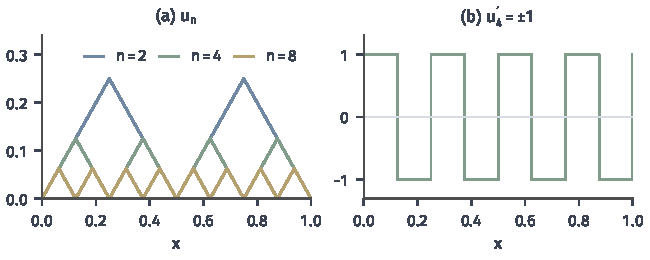
\includegraphics[width=110mm]{figures/03-optimization-evolution-and-signals/01-optimization/matplotlib/c9-bolza-sawtooth/figure.pdf}
  \caption{取不到下确界的最小化序列。(a)~斜率为$\pm1$、齿高$1/(2n)$的锯齿$u_n$，$n=2,4,8$，在$J(u)=\int_0^1((u'^2-1)^2+u^2)\,dx$下$J(u_n)=1/(12n^2)$；(b)~$u_4'$在$\pm1$间交替。$u_n$一致趋于零，$u_n'$弱收敛到零但$|u_n'|$恒为$1$，弱极限$0$的目标值为$1$。}
  \label{fig:opt-fn-bolza-sawtooth}
\end{figure}

两个例子中的目标都连续，下水平集也有界，可见目标连续不足以单独保证达到下确界。缺失的是目标在弱极限下的行为：能量可以藏进振荡或越来越远的坐标中，在弱极限里消失，而目标并不因此变小。

\paragraph{需要逐项检查的三件事}
按极限论证的步骤，问题分成三个。第一，最小化序列能否保持有界；第二，能否从中选出某种意义下收敛的子列；第三，极限是否仍可行，且目标值不超过序列目标值的下极限。第二步在Hilbert空间中由卷二已证明的结论提供：Hilbert空间中的每个有界序列都有弱收敛的子列，即存在$u$使$\langle w,u_{n_k}\rangle\to\langle w,u\rangle$对每个$w$成立，记作$u_{n_k}\rightharpoonup u$。同一处还证明了范数在弱极限下只能下降：$u_n\rightharpoonup u$推出$\|u\|\le\liminf_n\|u_n\|$。第一、三步则必须针对具体目标与约束检查。驻点方程有形式解，并不能反推出这些条件成立。

\subsection{直接法}
\label{sec:opt-fn-direct-method}

把三件事写成可以检查的条件，就得到下面的存在性定理。先给出两个与弱收敛配套的概念：若$u_n\in C$、$u_n\rightharpoonup u$总推出$u\in C$，称$C$\term{弱序列闭}（weakly sequentially closed）；若$u_n\rightharpoonup u$（均在$C$中）总推出$J(u)\le\liminf_nJ(u_n)$，称$J$在$C$上\term{弱序列下半连续}（weakly sequentially lower semicontinuous）。

\begin{theorem}[直接法]
\label{thm:opt-fn-direct-method}
设$H$为实Hilbert空间，$C\subseteq H$非空且弱序列闭，$J:H\to\mathbb R\cup\{+\infty\}$满足：
\begin{enumerate}
 \item 存在$u_0\in C$使$J(u_0)<+\infty$；
 \item 下水平集$S=\{u\in C:J(u)\le J(u_0)\}$有界；
 \item $J$在$C$上弱序列下半连续。
\end{enumerate}
则$J$在$C$上的下确界有限，并在某个$u^\star\in C$处达到。
\end{theorem}

\begin{proof}
记$m=\inf_CJ$，$m\le J(u_0)<+\infty$，暂不排除$m=-\infty$。

第一步，有界的最小化序列。取$u_n\in C$使$J(u_n)\to m$；去掉开头有限项后可设$J(u_n)\le J(u_0)$，于是$u_n\in S$，由条件2，$(u_n)$有界。

第二步，弱收敛子列。由Hilbert空间中有界序列的弱子列定理，存在子列$u_{n_k}\rightharpoonup u^\star$。

第三步，极限可行。$C$弱序列闭，所以$u^\star\in C$。

第四步，下极限比较。由条件3，$J(u^\star)\le\liminf_kJ(u_{n_k})=m$。$J$不取$-\infty$，所以$m>-\infty$；又$u^\star\in C$，$J(u^\star)\ge m$，故$J(u^\star)=m$。
\end{proof}

证明中“目标有下界”不是额外的假设，而是第四步的结论。条件2常由\term{强制性}（coercivity）得到：若$\|u\|\to\infty$（$u\in C$）时$J(u)\to+\infty$，则任何下水平集都有界。直接法只回答存在，不回答唯一。

\paragraph{唯一性另需凸性}
若$C$凸，$J$在$C$上严格凸，即$u\neq v$、$t\in(0,1)$时$J(tu+(1-t)v)<tJ(u)+(1-t)J(v)$，则最小点至多一个：设$u_1\neq u_2$都达到$m$，中点在$C$中且$J\bigl(\frac{u_1+u_2}2\bigr)<m$，矛盾。存在与唯一是两个独立的结论，分别由直接法与严格凸性提供。

\paragraph{如何检查弱序列闭与弱下半连续}
以下几条在例子中最常用。若$B:H\to Y$是到另一个Hilbert空间的有界线性算子，则$u_n\rightharpoonup u$推出$Bu_n\rightharpoonup Bu$，因为对每个$w\in Y$，$u\mapsto\langle w,Bu\rangle_Y$是$H$上的有界线性泛函。结合范数的弱下半连续性，$\frac12\|Bu-y\|_Y^2$在$H$上弱序列下半连续。由有限个有界线性泛函的等式或不等式$L_iu=c_i$、$L_iu\le c_i$定义的集合弱序列闭，因为弱收敛下每个$L_iu_n\to L_iu$。一般的闭凸集与凸下半连续目标同样满足这两条性质，这要用到下一小节的投影，届时再证明。

\paragraph{反面：非凸目标}
上一小节的两个例子都满足条件1与条件2，失败在条件3：$(\|\bm x\|_2^2-1)^2$与$(u'^2-1)^2$对$\bm x$或$u'$不凸，弱极限可以抬高它们的值。这说明一般非凸目标的范数连续性或范数下半连续性，都不能代替弱下半连续性。

\paragraph{反射空间（补充）}
证明中只有第二步用到Hilbert结构。卷二还证明了反射Banach空间中有界序列有弱收敛子列；$1<p<\infty$时$L^p$与$W^{1,p}$都是反射空间。在这样的空间中，把三个条件中的弱收敛按对偶空间理解，同样的四步证明照样成立。

\paragraph{导数平方能量满足全部条件}
回到章首的问题：$H=H^1(0,1)$，$C=\{u:u(0)=0,u(1)=1\}$，$J_0(u)=\frac12\|u'\|_{L^2}^2$。一维$H^1$中点值是有界线性泛函，所以$C$弱序列闭；$u\mapsto u'$是$H^1\to L^2$的有界线性算子，所以$J_0$弱序列下半连续。对$u\in C$，$|u(x)|=|\int_0^xu'\,dt|\le\|u'\|_{L^2}$，于是$\|u\|_{L^2}^2\le\|u'\|_{L^2}^2$，
\[
 \|u\|_{H^1}^2=\|u\|_{L^2}^2+\|u'\|_{L^2}^2\le4J_0(u) ,
\]
下水平集有界。直接法给出最小点存在，与第~\ref{sec:opt-fn-euler-lagrange}节直接验证的结果一致。高维区域上，起同样作用的是Poincaré不等式：在$H_0^1(\Omega)$中$\|u\|_{L^2}\le C_\Omega\|\nabla u\|_{L^2}$，因此固定边界迹时导数平方能量控制整个$H^1$范数。

\paragraph{线性增长的能量}
对第~\ref{sec:opt-fn-first-variation}节的平滑导数幅度~\eqref{eq:opt-fn-smoothed-tv}，情况不同。一维固定端点时，令$u_\delta$在$[\frac12-\frac\delta2,\frac12+\frac\delta2]$上从$0$线性升到$1$，其余位置为常数。它属于$C$，并且
\[
 \int_0^1|u_\delta'|\,dx=1,\qquad\int_0^1|u_\delta'|^2dx=\frac1\delta ,\qquad J_\varepsilon(u_\delta)\le\int_0^1(|u_\delta'|+\varepsilon)\,dx=1+\varepsilon .
\]
$\delta\to0$时$\|u_\delta\|_{H^1}\to\infty$，而目标值保持有界：下水平集在$H^1$中无界，条件2不成立（图~\ref{fig:opt-fn-transition-width}）。原因是$\psi_\varepsilon(p)$只随$|p|$线性增长，无法像平方那样惩罚越来越陡的过渡。检查失败并不证明最小点不存在：这个一维问题中，$\psi_\varepsilon$凸，由Jensen不等式$J_\varepsilon(u)\ge\psi_\varepsilon\bigl(\int_0^1u'\,dx\bigr)=\sqrt{1+\varepsilon^2}=J_\varepsilon(x)$，直线仍是最小点。但在一般问题中，陡峭过渡的极限是跳跃，它已不在$H^1$中。允许跳跃需要换到有界变差函数等新空间，附加平方增长项则改变了目标；两种处理都须重新核验条件，本书不展开有界变差空间的存在理论。

\begin{figure}[!htb]
  \centering
  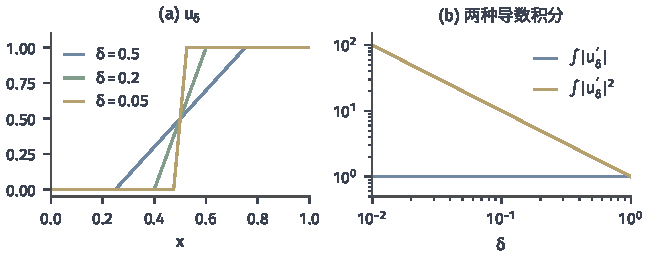
\includegraphics[width=110mm]{figures/03-optimization-evolution-and-signals/01-optimization/matplotlib/c9-transition-width/figure.pdf}
  \caption{宽度为$\delta$的单位过渡。(a)~在$x=1/2$附近宽$\delta=0.5,0.2,0.05$的区间内从$0$线性升到$1$的$u_\delta$；(b)~导数幅度积分$\int|u_\delta'|$恒为$1$（蓝），导数平方积分$\int|u_\delta'|^2=1/\delta$随$\delta\to0$增长（黄），两轴均为对数。线性增长的能量不能阻止过渡变陡。}
  \label{fig:opt-fn-transition-width}
\end{figure}

\subsection{闭凸集投影}
\label{sec:opt-fn-projection}

第~\ref{chap:opt-nonsmooth}章把有限维闭凸集上的投影作为邻近映射的特例建立起来，第~\ref{chap:constrained-optimization}章用它构造约束迭代。在一般Hilbert空间中，“离给定元素最近的可行点”同样是一个泛函最小化问题。它的结构足够好，可以不借直接法，只用完备性和平行四边形恒等式完整证明存在唯一。

\begin{theorem}[闭凸集上的投影]
\label{thm:opt-fn-projection}
设$H$为实Hilbert空间，$C\subseteq H$非空、闭且凸，$z\in H$。则存在唯一的$p\in C$使
\[
 \|z-p\|_H=\inf_{u\in C}\|z-u\|_H .
\]
记$p=\Pi_Cz$，称为$z$在$C$上的\term{投影}（projection）。
\end{theorem}

\begin{proof}
记$d=\inf_{u\in C}\|z-u\|_H$，取$u_n\in C$使$\|z-u_n\|_H\to d$。

第一步，最小化序列是Cauchy列。对$z-u_n$与$z-u_k$用平行四边形恒等式，
\[
 \|u_n-u_k\|_H^2=2\|z-u_n\|_H^2+2\|z-u_k\|_H^2-4\Bigl\|z-\frac{u_n+u_k}2\Bigr\|_H^2 .
\]
$C$凸，中点$\frac{u_n+u_k}2\in C$，所以最后一项的范数平方至少为$d^2$。于是$\|u_n-u_k\|_H^2\le2\|z-u_n\|_H^2+2\|z-u_k\|_H^2-4d^2\to0$。

第二步，极限可行。$H$完备，$u_n$收敛到某个$p$；$C$闭，$p\in C$；由范数连续，$\|z-p\|_H=d$。

第三步，唯一。若$p_1,p_2\in C$都达到$d$，对它们用同一个恒等式，$\|p_1-p_2\|_H^2\le2d^2+2d^2-4d^2=0$。
\end{proof}

凸性在证明中出现了两次：中点留在$C$中，既让最小化序列成为Cauchy列，又排除了两个不同的最近点。完备性与闭性则保证极限存在且可行。闭线性子空间上的正交投影有同样结构的证明，见\BookChapterRef{chap:function-spaces}{卷二“函数空间”章}；那里中点留在子空间中，这里改用凸性保证同一件事。

\paragraph{钝角刻画}
投影点满足一个只涉及内积的条件，它是变分不等式~\eqref{eq:opt-fn-variational-inequality}的特例。

\begin{theorem}[投影的变分刻画]
\label{thm:opt-fn-projection-characterization}
在定理~\ref{thm:opt-fn-projection}的条件下，$p\in C$等于$\Pi_Cz$，当且仅当
\begin{equation}
 \langle z-p,u-p\rangle_H\le0\qquad\text{对所有}u\in C .
 \label{eq:opt-fn-projection-vi}
\end{equation}
\end{theorem}

\begin{proof}
必要性：$J(u)=\frac12\|z-u\|_H^2$在$H$上Fréchet可微，$DJ(p)[h]=\langle p-z,h\rangle_H$，由定理~\ref{thm:opt-fn-variational-inequality}(1)，$\langle p-z,u-p\rangle_H\ge0$，即~\eqref{eq:opt-fn-projection-vi}。充分性：对$u\in C$展开
\[
 \|z-u\|_H^2=\|z-p\|_H^2-2\langle z-p,u-p\rangle_H+\|u-p\|_H^2\ge\|z-p\|_H^2 .
\]
\end{proof}

几何上，~\eqref{eq:opt-fn-projection-vi}说$z-p$与从$p$指向$C$中任一点的向量夹角不小于直角（图~\ref{fig:opt-fn-projection-geometry}(a)）。若$C$是闭线性子空间$M$，取$u=p\pm w$（$w\in M$），两个不等式合起来给出$\langle z-p,w\rangle_H=0$：钝角条件加强为正交条件（图~\ref{fig:opt-fn-projection-geometry}(b)），回到卷二的正交投影。

\begin{figure}[!htb]
  \centering
  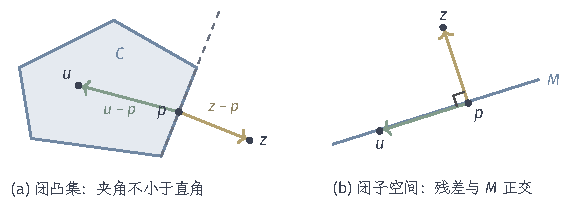
\includegraphics[width=96.725mm]{figures/03-optimization-evolution-and-signals/01-optimization/tikz/c9-projection-geometry/figure.pdf}
  \caption{Hilbert空间中投影的几何（平面示意）。(a)~闭凸集$C$（浅蓝）外一点$z$的投影$p$：残差$z-p$（黄）与任一$u-p$（绿）的夹角不小于直角，虚线为过$p$且与$z-p$垂直的支撑线；(b)~闭子空间$M$上，$u$可沿$M$向两侧取，钝角条件变为残差$z-p$与$M$正交。}
  \label{fig:opt-fn-projection-geometry}
\end{figure}

\paragraph{非扩张性}
对$z_1,z_2\in H$，记$p_i=\Pi_Cz_i$。在~\eqref{eq:opt-fn-projection-vi}中分别取$(z,p,u)=(z_1,p_1,p_2)$与$(z_2,p_2,p_1)$，两式相加得$\langle(z_1-z_2)-(p_1-p_2),p_2-p_1\rangle_H\le0$，即
\[
 \|p_1-p_2\|_H^2\le\langle z_1-z_2,p_1-p_2\rangle_H\le\|z_1-z_2\|_H\|p_1-p_2\|_H .
\]
所以$\|\Pi_Cz_1-\Pi_Cz_2\|_H\le\|z_1-z_2\|_H$：投影不放大距离，称为非扩张。这与有限维中的性质相同，证明也只用了内积。

\paragraph{闭凸集弱序列闭}
钝角刻画回答了上一小节留下的问题。设$C$非空闭凸，$u_n\in C$，$u_n\rightharpoonup u$。令$p=\Pi_Cu$，由~\eqref{eq:opt-fn-projection-vi}，$\langle u-p,u_n-p\rangle_H\le0$对每个$n$成立；令$n\to\infty$，由弱收敛得$\langle u-p,u-p\rangle_H\le0$，所以$u=p\in C$。进一步，若$J$凸且（按范数）下半连续，则每个下水平集$\{J\le c\}$闭且凸，因而弱序列闭。设$u_n\rightharpoonup u$而$J(u)>\liminf_nJ(u_n)$，取$c$严格介于两者之间，则有子列始终落在$\{J\le c\}$中，其弱极限$u$也在其中，$J(u)\le c$，矛盾。所以凸且下半连续的目标弱序列下半连续，直接法的条件3对它自动成立。

\paragraph{检查候选集}
均值约束$C=\{u\in L^2(0,1):\int_0^1u\,dx=1\}$是有界线性泛函$u\mapsto\int_0^1u$的一个水平集，闭且凸。它的投影是$\Pi_Cz=z+(1-\int_0^1z)\cdot\mathbf 1$：残差$z-\Pi_Cz$为常数，与$C$中任意两元之差（均值为零）正交，满足~\eqref{eq:opt-fn-projection-vi}且等号成立。例如$z(x)=x$时$\Pi_Cz=x+\frac12$。点值约束则要小心：在$L^2(0,1)$的等价类上，“$u(1/2)=0$”没有意义，因为改变一个零测集上的值不改变元素；只有在点值是连续线性泛函的空间中（如一维$H^1$）才能用这样的约束定义闭凸集。

\paragraph{凸性与闭性不能省}
非凸集合可能有多个最近点：在单位球面$\{\|u\|_H=1\}$上，零元到每一点的距离都是$1$。也可能一个都没有：在$\ell^2$中取$C=\{(1+\frac1k)\bm e_k:k\ge1\}$，任两点距离大于$\sqrt2$，所以$C$闭；零元到$C$的距离下确界为$1$，却没有哪一点距离恰为$1$。有限维中的投影算法因此不能不加条件地当成无限维的求解保证：可行集的闭性与凸性都要先在所选空间中核实。
